\documentclass[11pt,a4paper]{article}
\usepackage[margin=18mm]{geometry}
\usepackage{amsmath,amssymb,mathtools}
\usepackage{booktabs,array,enumitem}
\usepackage[dvipsnames]{xcolor}
\usepackage{graphicx,listings,tikz,float,needspace}
\usetikzlibrary{arrows.meta,positioning}
\usepackage[most]{tcolorbox}
\usepackage{hyperref}
\hypersetup{colorlinks=true,urlcolor=MidnightBlue,linkcolor=MidnightBlue}
\setlength{\parindent}{0pt}\setlength{\parskip}{4pt}
\newcommand{\course}{PHY4605 Computational Methods in Physics}
\newcommand{\units}[1]{\,\mathrm{#1}}
\newtcolorbox{keybox}{colback=RoyalBlue!5,colframe=RoyalBlue!65!black,boxrule=.7pt,arc=2mm}
\newtcolorbox{checkbox}{colback=ForestGreen!5,colframe=ForestGreen!55!black,boxrule=.7pt,arc=2mm}
\newtcolorbox{aibox}{colback=BurntOrange!7,colframe=BurntOrange!80!black,boxrule=.7pt,arc=2mm}
\lstdefinestyle{matlabstyle}{language=Matlab,basicstyle=\ttfamily\footnotesize,keywordstyle=\color{RoyalBlue!75!black},commentstyle=\color{ForestGreen!55!black},stringstyle=\color{BurntOrange!80!black},numbers=left,numberstyle=\scriptsize\color{black!50},numbersep=5pt,frame=single,rulecolor=\color{RoyalBlue!25},backgroundcolor=\color{RoyalBlue!3},showstringspaces=false,columns=fullflexible,keepspaces=true,breaklines=true}
\begin{document}
{\large\textsc{\course}}\\[-2pt]
{\small Learning Note \textbar\ Week 2}\par\vspace{4pt}
{\LARGE\bfseries Pseudocode, Loops, and Debugging}\par\vspace{3pt}
\textit{Turn one familiar physics equation into a sequence that can be traced, checked, and repaired.}

\begin{keybox}\textbf{Physical question.} A ball is launched straight upward. We already know its position equation. How can we make MATLAB calculate one position at a time in an order that another person can trace and verify?\end{keybox}

\section*{Core learning outcomes}
\begin{enumerate}[nosep,leftmargin=5mm]
\item decompose a familiar physics calculation into short pseudocode;
\item trace, complete, and modify a simple indexed \texttt{for} loop; and
\item diagnose a clear defect using code evidence, one known-value check, and physical reasoning.
\end{enumerate}

\section*{How to use this note}
Read the physical claim first, then the pseudocode, then the MATLAB fragment. Pause at each trace or prediction checkpoint before looking at the supplied result. The aim is not to memorise loop punctuation; it is to make every computational step explainable.

\section*{1. Reuse a familiar physical model}
Choose upward as positive, neglect air resistance, and take gravity to be constant. The vertical position is
\[
y(t)=y_0+v_0t-\frac{1}{2}gt^2.
\]
In words: \emph{position equals the starting position plus the upward launch contribution minus the downward gravity contribution}.

\begin{center}
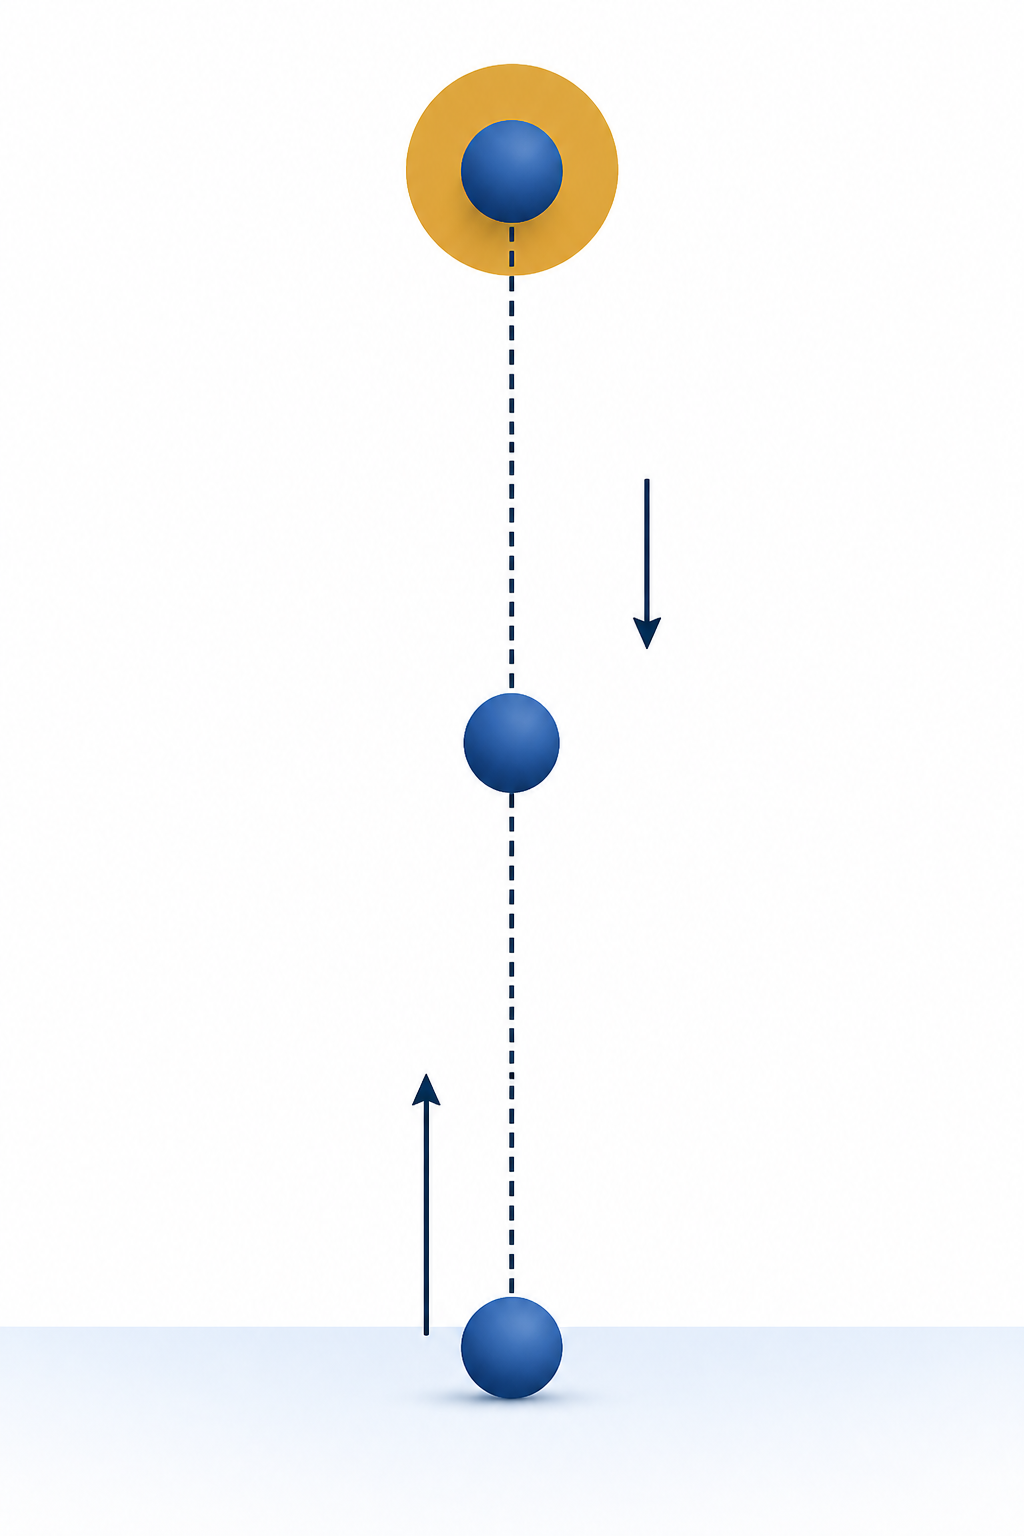
\includegraphics[height=52mm]{../lecture-slides/assets/vertical-launch-matte.png}
\end{center}
\begin{center}\small Familiar vertical launch: the geometry is one-dimensional, so the computational focus can stay on the algorithm.\end{center}

\begin{center}\small\begin{tabular}{>{\raggedright\arraybackslash}p{.18\linewidth}>{\raggedright\arraybackslash}p{.26\linewidth}>{\raggedright\arraybackslash}p{.43\linewidth}}\toprule
\textbf{Physics symbol} & \textbf{MATLAB name} & \textbf{Meaning and unit}\\ \midrule
$y(t)$ & \texttt{y\_m} & vertical position, m\\
$t$ & \texttt{t\_s} & ordered time samples, s\\
$y_0$ & \texttt{y0\_m} & starting position, m\\
$v_0$ & \texttt{v0\_mps} & upward launch velocity, m s$^{-1}$\\
$g$ & \texttt{g\_mps2} & gravity magnitude, m s$^{-2}$\\ \bottomrule
\end{tabular}\end{center}

Use $y_0=0\units{m}$, $v_0=20\units{m\,s^{-1}}$, $g=9.81\units{m\,s^{-2}}$, and times from $0$ to $4\units{s}$ in $0.5\units{s}$ steps.

\begin{checkbox}\textbf{Prediction checkpoint.} The ball should rise, slow, reach a highest point, and then fall. At $t=0$, the model must return $y=0\units{m}$.\end{checkbox}

\section*{2. Decompose before writing MATLAB}
Separate the task into four jobs before thinking about syntax.

\begin{center}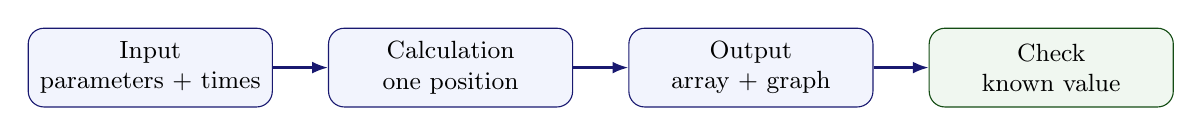
\begin{tikzpicture}[node distance=8mm and 7mm,every node/.style={font=\small,align=center},box/.style={draw=MidnightBlue,rounded corners=2mm,fill=RoyalBlue!7,minimum width=31mm,minimum height=10mm},check/.style={draw=ForestGreen!55!black,rounded corners=2mm,fill=ForestGreen!7,minimum width=31mm,minimum height=10mm},arrow/.style={-{Latex[length=2mm]},thick,MidnightBlue}]
\node[box] (in) {Input\\parameters + times};
\node[box,right=of in] (calc) {Calculation\\one position};
\node[box,right=of calc] (out) {Output\\array + graph};
\node[check,right=of out] (chk) {Check\\known value};
\draw[arrow] (in)--(calc);\draw[arrow] (calc)--(out);\draw[arrow] (out)--(chk);
\end{tikzpicture}\end{center}

This decomposition is already an algorithm map. It answers \emph{what must happen} before MATLAB answers \emph{how to write it}.

\section*{3. Write guided pseudocode}
One sensible pseudocode sequence is:
\begin{enumerate}[nosep,leftmargin=7mm]
\item store $y_0$, $v_0$, $g$, and the ordered time samples;
\item make one empty position slot for every time;
\item start at the first MATLAB index;
\item read the current time;
\item calculate one position and store it in the matching slot;
\item move to the next index and repeat until the final time; and
\item plot, check, and interpret the result.
\end{enumerate}

\begin{keybox}\textbf{Key idea.} Pseudocode is not a rough version of MATLAB punctuation. It is a readable description of the calculation order.\end{keybox}

\section*{4. A loop is a controlled repeated update}
The time array and parameters are declared before the loop.
\begin{lstlisting}[style=matlabstyle,caption={Locked inputs for the lecture example}]
y0_m = 0;
v0_mps = 20;
g_mps2 = 9.81;
t_s = 0:0.5:4;
n_samples = numel(t_s);
\end{lstlisting}

Preallocation creates the matching output array before the loop starts:
\begin{lstlisting}[style=matlabstyle,caption={Preallocate one storage slot per time sample}]
y_m = zeros(size(t_s));
\end{lstlisting}

Inside the loop, the currently selected time is a scalar. Ordinary scalar multiplication and powers are therefore appropriate.
\Needspace{9\baselineskip}
\begin{lstlisting}[style=matlabstyle,caption={One position is calculated and stored on each pass}]
for sample_index = 1:n_samples
    current_time_s = t_s(sample_index);
    y_m(sample_index) = y0_m + v0_mps*current_time_s ...
        - 0.5*g_mps2*current_time_s^2;
end
\end{lstlisting}

The five pieces to look for are: \textbf{start}, \textbf{current value}, \textbf{update}, \textbf{matching storage location}, and \textbf{stopping point}.

\section*{5. Trace the first two passes by hand}
Do not begin by staring at the whole loop. Follow one index at a time.

\begin{center}\small\begin{tabular}{>{\raggedright\arraybackslash}p{.16\linewidth}>{\raggedright\arraybackslash}p{.20\linewidth}>{\raggedright\arraybackslash}p{.27\linewidth}>{\raggedright\arraybackslash}p{.25\linewidth}}\toprule
\textbf{Pass} & \textbf{Index} & \textbf{Current time} & \textbf{Stored position}\\ \midrule
1 & \texttt{sample\_index=1} & \texttt{t\_s(1)=0.0 s} & \texttt{y\_m(1)=0.00000 m}\\
2 & \texttt{sample\_index=2} & \texttt{t\_s(2)=0.5 s} & \texttt{y\_m(2)=8.77375 m}\\ \bottomrule
\end{tabular}\end{center}

\begin{checkbox}\textbf{Trace checkpoint.} Why does index 2 mean $0.5\units{s}$ rather than $2\units{s}$? Because MATLAB indexing counts storage locations; the stored values are set by the time array.\end{checkbox}

\section*{6. Bounded completion instead of blank-page coding}
Suppose the loop scaffold is supplied as
\begin{lstlisting}[style=matlabstyle,caption={Complete only the missing calculation}]
for sample_index = 1:n_samples
    current_time_s = t_s(sample_index);
    y_m(sample_index) = ______________________________;
end
\end{lstlisting}

Translate the current step back into words: \emph{use the current time, calculate one vertical position, and store it in the matching location}. The completed expression is
\begin{lstlisting}[style=matlabstyle]
y0_m + v0_mps*current_time_s - 0.5*g_mps2*current_time_s^2
\end{lstlisting}

\section*{7. Read the output, then modify one input}
The retained MATLAB evidence uses exactly the same loop with $v_0=20\units{m\,s^{-1}}$ and then with only the launch speed changed to $15\units{m\,s^{-1}}$.

\begin{figure}[H]
\centering
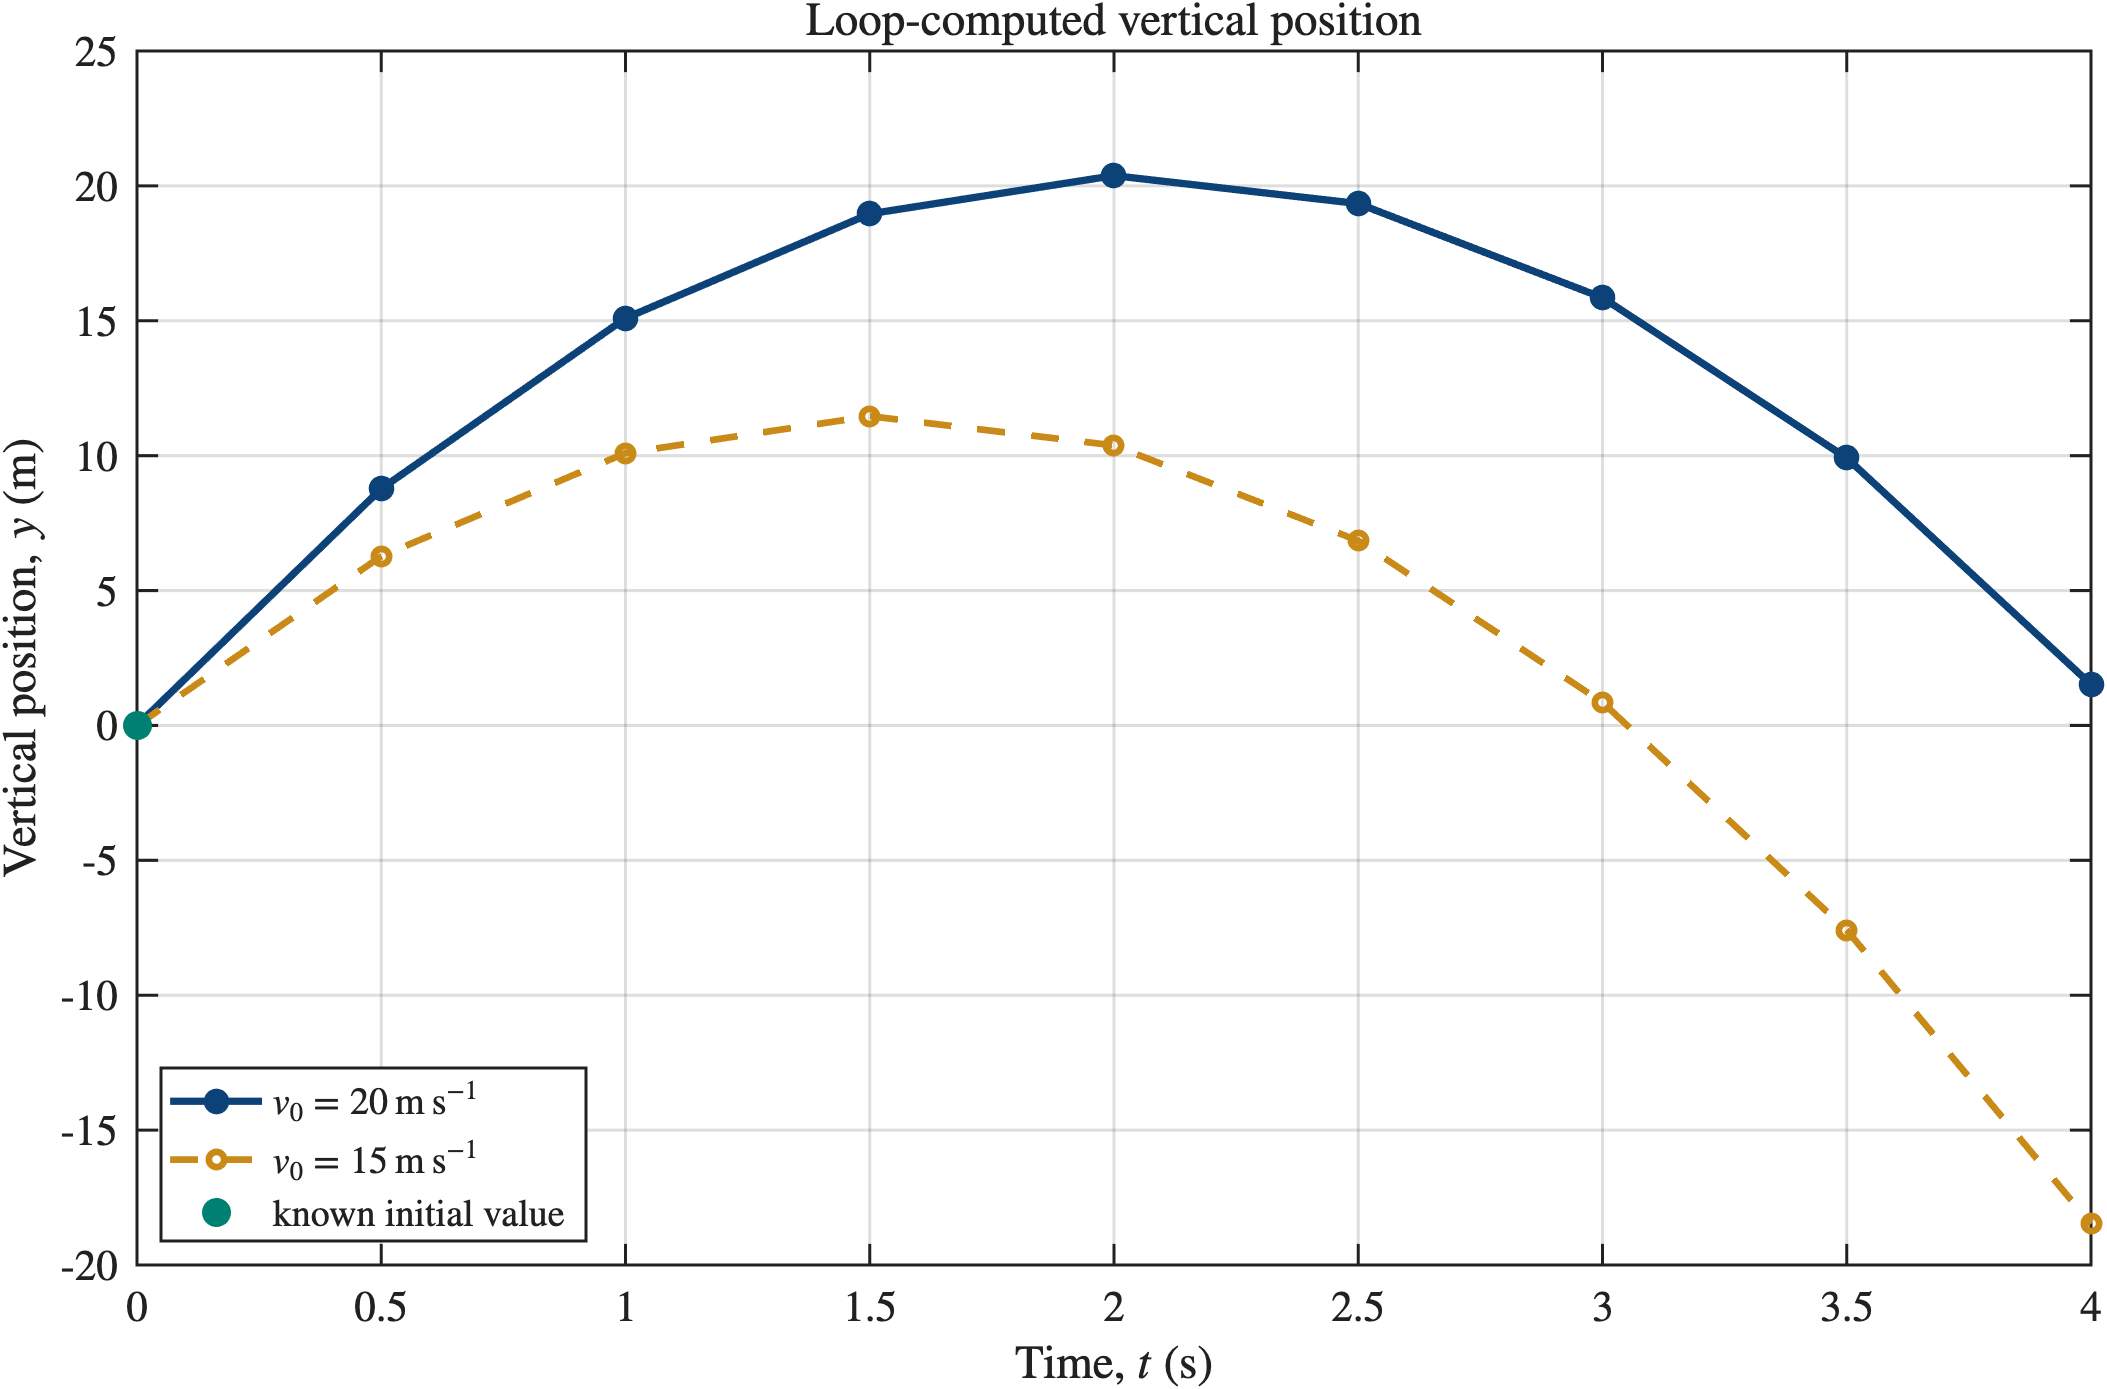
\includegraphics[width=.72\linewidth]{../matlab/assets/week02_loop_position.png}
\caption{Loop-computed vertical position for the locked lecture model. The lower launch speed produces a lower sampled peak while the initial value remains unchanged.}
\end{figure}

\begin{checkbox}\textbf{Parameter prediction.} Before running the second loop, predict that lowering $v_0$ reduces the maximum height. Only the launch-speed input changes; the loop structure does not.\end{checkbox}

\section*{8. One Core validation: the known initial value}
At the first stored time, $t=0$, the model must reproduce its stated initial condition. This value is known before the loop runs.
\begin{lstlisting}[style=matlabstyle,caption={Executable initial-value validation}]
assert(abs(y_m(1)-y0_m) < 1e-12, ...
    'Initial-position validation failed.')
\end{lstlisting}

\begin{checkbox}\textbf{Validation result.} The first stored value is $y(0)=0\units{m}$, matching $y_0=0\units{m}$. The assertion passes in a fresh MATLAB session.\end{checkbox}

The check is powerful but not magical. A wrong gravity sign still gives $y(0)=0$ because the time-dependent terms vanish at zero. That defect needs physical reasoning as well.

\section*{9. Debug by classifying the defect}
Different defects need different evidence.

\begin{center}\small\begin{tabular}{>{\raggedright\arraybackslash}p{.24\linewidth}>{\raggedright\arraybackslash}p{.31\linewidth}>{\raggedright\arraybackslash}p{.34\linewidth}}\toprule
\textbf{Defect type} & \textbf{What you may observe} & \textbf{Useful first evidence}\\ \midrule
Syntax & MATLAB cannot complete the code structure & error location, surrounding punctuation, missing \texttt{end}\\
Array/indexing/operator & code may run but reads/stores the wrong values & index-to-array mapping, sizes, selected entries, operator meaning\\
Physical/logical & code runs but implements the wrong physics & sign convention, units, prediction, known or limiting behaviour\\ \bottomrule
\end{tabular}\end{center}

Use the MATLAB error location when MATLAB supplies one, but do not stop there. Compare the line with the pseudocode and physical model.

\subsection*{Indexing example}
This loop repeatedly overwrites only the first storage location:
\Needspace{10\baselineskip}
\begin{lstlisting}[style=matlabstyle]
y_index_defect_m = zeros(size(t_s));
for sample_index = 1:n_samples
    current_time_s = t_s(sample_index);
    y_index_defect_m(1) = y0_m + v0_mps*current_time_s ...
        - 0.5*g_mps2*current_time_s^2;
end
\end{lstlisting}
The repair is to store the current result in \texttt{y\_index\_defect\_m(sample\_index)} so each time has a matching position slot.

\subsection*{Physical-sign example}
The line below is legal MATLAB but contradicts the upward-positive model:
\begin{lstlisting}[style=matlabstyle]
y_wrong_sign_m(sample_index) = y0_m + v0_mps*current_time_s ...
    + 0.5*g_mps2*current_time_s^2;
\end{lstlisting}
The positive gravity contribution makes the computed trajectory bend upward. The correct model subtracts the gravity term because gravity points downward while upward is positive.

\begin{aibox}\textbf{Debugging caution.} ``The code ran'' is not validation. A physically wrong expression can produce smooth, plausible-looking numbers without any MATLAB error.\end{aibox}

\subsection*{Working exposure: loop and vectorised forms}
The analytical model can also be evaluated with one vectorised expression:
\begin{lstlisting}[style=matlabstyle]
y_vectorised_m = y0_m + v0_mps.*t_s - 0.5*g_mps2.*t_s.^2;
\end{lstlisting}
Here \texttt{t\_s} is an array, so element-wise operators are required. In the explicit loop, \texttt{current\_time\_s} is a scalar. The two forms should agree numerically for the same model and inputs.

\subsection*{Optional stretch: package the calculation as a function}
A distinction-level extension is to write a reusable function that accepts the model inputs and returns the position array, then design a second independent test. This is not required for the Core Week 2 route.

\section*{Three takeaways}
\begin{enumerate}[nosep,leftmargin=6mm]
\item Pseudocode makes the order of a computation visible before MATLAB syntax is introduced.
\item A traceable loop connects one index, one current input, one calculation, and one matching output slot.
\item Debugging combines code evidence with validation and physical reasoning; successful execution alone is not proof of correctness.
\end{enumerate}

\begin{keybox}\textbf{Preparation for the practical.} Be ready to transfer the same loop pattern to cooling, radioactive decay, and oscillation. For each context, state the model and units, trace the first passes, validate a known value, and record what any AI assistance changed or did not change.\end{keybox}

\end{document}
